% WSArena paper skeleton (IEEE two-column). Numbers and tables are generated into paper/gen/*.tex by scripts/make_paper_tables.py (not typed by hand).
% Engine: none installed yet (pdflatex/tectonic absent; download of tectonic was declined by the host). Source is kept compile-ready.
\documentclass[conference]{IEEEtran}
\usepackage{graphicx,booktabs,amsmath,amssymb,cite,url,siunitx}
\begin{document}
\title{WSArena: Can a Language Model Fix a Neural Network by Writing Its Weights?}
\author{\IEEEauthorblockN{Anonymous for now}\IEEEauthorblockA{authors and affiliations are filled in at release}}
\maketitle

\begin{abstract}
Recent demonstrations show that a language model can read the weights of a small network as text and edit them to fix a fault, with no gradients. These demonstrations use one model, a few runs and no controls, so it is hard to say what they show. We present WSArena, a benchmark for this task with a fixed protocol, checkpoints whose faults are known, a ladder of scripted controls, hidden test episodes, and diagnostics that ask whether the gains depend on reading the weights. In a pre-registered study of Claude Sonnet 5.5 and Opus 5.5 on 33 checkpoints from two task families (a small control suite and Meta-World), every editor beats random edits, which is a low bar because random edits lower the success rate. Against a closed-form refit that uses expert labels, the editors are not distinguishable on the control suite (10 checkpoints; this is not evidence of equality) and clearly worse on Meta-World, where Opus only matches a one-parameter gain search. In an exploratory ablation on eight control-suite checkpoints, hiding the weight values changes the gain by $+0.006$ on average (checkpoint-clustered 95\% CI $-0.115$ to $+0.115$), with large differences of both signs between checkpoints; we find no average benefit from seeing the values. The run-to-run standard deviation of an editor's gain on a fixed checkpoint is about 0.13 on the control suite and 0.08 on Meta-World, driven by a few large reversals, so single runs should not be used to rank models. We release the protocol, checkpoints, controls and analysis code.
\end{abstract}

\section{Introduction}
Weight-space programming asks a language model to change what a neural network does by writing its weights directly: no loss, no optimiser, no gradient. Early reports are striking: a model rewrites a few units of a policy and the policy goes from failing to succeeding~\cite{takehi2026sparks}. But a single successful edit says little. It could come from reading the weights, from knowing the task, from a lucky guess, or from a change that any rescaling would have made. Without hidden test episodes, repeated runs and cheap alternatives to compare against, none of these can be told apart.

WSArena turns the question into a measurement. We fix the protocol (four rounds, 16 development episodes per round, hidden episodes that are never fed back), use checkpoints whose faults are planted or known, and compare every editor with scripted controls that range from random edits to a closed-form refit and an oracle. We add diagnostics for what the editor actually did: what kind of edit it made, whether it needed to see the weights, and what it cost.

Our contributions are: (i) the protocol, checkpoints, controls and audit tooling, released with a frozen contract; (ii) a pre-registered study of two Claude models on 33 checkpoints, with analysis scripts fixed before the data existed; (iii) exploratory evidence that on these networks the gains show no average dependence on reading the weights, and a measurement of run-to-run noise, which is large enough to matter; (iv) a probe track for networks too large to print.

\section{Related Work}
\textbf{Weight-space programming.} Takehi et al.~\cite{takehi2026sparks} showed that a frontier language model can read, diagnose and edit the weights of small networks, and build some networks from scratch, without gradients. Their experiments are demonstrations: one model, mostly single runs, with the tools and feedback varying from task to task. Independent replications have started to appear. OpenWSP~\cite{openwsp2026} provides open tooling around a weight kernel, a forward-pass service and a versioned edit format, and reports that its own repair run on a language model scored well below the original, while stating that the two numbers are not comparable. Huang~\cite{huang2026break} reproduces several of the game-policy results and probes them with permuted input rows and shuffled hidden units; the same post notes that a model at maximum reasoning effort can spend its whole output budget thinking and never answer. A research note from Playground~\cite{playground2026robotics} extends the idea to robot policies with millions of weights and to a 3.35-billion-parameter vision-language-action model, with a numpy sandbox and a read-only probe; its authors call one of the headline gains unconfirmed after a repeatable second pass.

\textbf{Limits and controls.} Two preprints ask what the models actually use. Nusrat and Nusrat~\cite{nusrat2026clinical} have Claude audit small clinical-screening networks with planted flaws and find that it names the broken rule in most of them, but also that a simple statistic chosen for each flaw type finds the same flaws. Ahmed~\cite{ahmed2026reason} reports that a model reading a 125\,000-parameter CNN as text draws useful inferences from BatchNorm statistics and output-layer signs, but misreads dataset semantics in several cases; the results are exploratory and mostly single runs. WeightLoop~\cite{li2026weightloop} has the model write a reusable parameter-editing program that is then applied without further model calls, and compares it with random edits.

\textbf{Where WSArena fits.} These studies differ in tools, output budget, feedback, network size and baselines, so their numbers cannot be lined up. WSArena fixes the protocol, uses checkpoints whose faults are known, ranks every model against cheap and privileged controls, repeats runs so that run-to-run noise can be measured, and adds two ablations aimed at the question the controls raise: do the gains depend on reading the weights at all (blind and shuffled prompts), and do they survive a function-preserving rearrangement of the weights.

\section{The Task}
\subsection{What the model does}
The model receives a small multilayer perceptron policy as plain text: every weight, rounded to five significant digits, plus a description of the environment and its success rule. It answers with a short analysis and one block of edits. An edit is a numpy-style statement such as \texttt{W3[:, 1] *= 2} or \texttt{b1[0:4] = -1}; \texttt{RESET} restores the original weights. Only the last block of a reply is read, statements that cannot be parsed are skipped and counted, and nothing is executed. The model has no tools, no code execution, no data, no loss and no optimiser.

A run has four rounds. After each round the edited policy is run on 16 fresh development episodes and the model sees a short JSON report: success rate, mean return, a count of failure types and a few diagnostics. The weights after the fourth round are scored on 200 hidden in-distribution episodes and 200 hidden out-of-distribution episodes, which are never fed back. There are no retries. A round in which the model produces no usable edit stays in the denominator as ``no change''.

\subsection{Checkpoints with known ground truth}
Every run starts from a stored checkpoint, addressed by the SHA-256 of its weights. We use four classes. \emph{S0} is an all-zero network. \emph{S1} is a healthy network with a planted fault (a weak action axis, a bias shift or a flipped unit) whose location we keep as ground truth. \emph{S2} is a network that fails on its own, for example because it was cloned from flawed demonstrations. \emph{S3} is a healthy network that still has room to improve. Each class is accepted only if its success rate on a separate selection split falls inside a pre-set band. Selection, development, hidden-ID and hidden-OOD episodes use disjoint seed ranges. Combinations we could not build are listed as infeasible rather than dropped silently.

\subsection{Controls}
A model's gain only means something next to what cheap procedures achieve. We run, on the same checkpoints and the same development budget: no edit; random sparse perturbations; greedy random edits; a one-knob gain search; a per-tensor gain search; a hand-compiled PD controller; a closed-form refit that sees expert labels (privileged); and an oracle that restores the original weights (privileged, S1 only). The two privileged controls are reported but never ranked against the model.

\section{Metrics and Statistics}
The main outcome is the change in hidden success rate, $\Delta\mathrm{SR}$, between the edited and the unedited policy on the same 200 episodes. The unit of inference is the checkpoint: repeated runs are averaged inside a checkpoint and episodes are never treated as independent samples. We compare arms with paired, task-stratified bootstrap intervals and sign-flip tests, and correct the pre-registered family of twelve primary tests with the Holm procedure. Evaluation is deterministic given weights and seeds; the episode-sampling noise floor, measured on disjoint episode sets, has a median standard deviation of 0.03, and we treat changes below 0.10 as indistinguishable from no change.

Beyond success rate we record four diagnostics. The \emph{edit mechanism} (scale, low-rank, local, layer rewrite, rewrite) is read off the weight difference. The \emph{weight-reliance index} compares $\Delta\mathrm{SR}$ with the real weights against $\Delta\mathrm{SR}$ when the weight values are hidden or shuffled. The \emph{permutation sensitivity} compares the gain on a checkpoint and on a function-preserving re-arrangement of its units. Finally we log tokens, time and cost for every run, and compare against trained networks under a resource ledger.

\section{Experiments}
\subsection{Setup}
We test Claude Sonnet 5.5 and Opus 5.5 through the Claude Code command line client on a subscription, with all tools, memory and project instructions switched off, and a neutral working directory. Each turn is a stateless call. Every run is checked for tool use and for identity leaks in the prompt and the raw event stream. The primary study uses checkpoints built from seeds 2 and 3 only; seed 1 was used in a pilot and in diagnostics and is never part of the primary analysis. The task families are a small control suite (reach, avoid, hold, delay; networks with 24 hidden units and 0.8--1k parameters) and three Meta-World manipulation tasks. The analysis script for the pre-registered comparisons (C1 to C3, plus a secondary family against the strongest simple controls) was committed before the first run; the diagnostics reported below (weight reliance, run-to-run spread, attempt rates) were written afterwards and are exploratory.

The unit of inference is the checkpoint. We use paired, task-stratified bootstrap intervals and sign-flip tests, and correct the twelve (control suite) or six (Meta-World) pre-registered tests with the Holm procedure. The intervals in the tables resample checkpoints within tasks and are therefore conditional on the tasks; unstratified cluster intervals are wider (for Sonnet-medium against the closed-form refit on the control suite, $[-0.14, +0.45]$ instead of $[-0.09, +0.38]$) and are given in the released addendum.

\subsection{Main results}
Table~\ref{tab:t0} and Table~\ref{tab:mw} give the pre-registered comparisons; Figure~\ref{fig:main} shows every checkpoint. All editors beat random edits by a wide margin, but that is a low bar: random edits lower the success rate by 0.26 to 0.30 on faulty checkpoints. The informative comparisons are against doing nothing and against the simple controls. The picture against the closed-form refit, which sees expert labels, differs between the two families. On the control suite the editors are not distinguishable from it (Holm $p$ from 0.31 to 0.50); with 10 checkpoints the study could detect a difference of about 0.18, so this is a lack of evidence of a difference, not evidence that they are equal. On Meta-World both editors are clearly worse: $-0.35$ for Sonnet and $-0.22$ for Opus (Holm $p=0.024$), and Opus only matches the one-parameter gain search. On healthy checkpoints (S3) the editors gain little, except Opus on the control suite. The S3-minus-L2 contrast in the tables is negative largely because healthy checkpoints have little headroom; it is not a measure of capability.

\begin{table}[t]
\centering
\caption{Tier-0, pre-registered comparisons (16 checkpoints; L2 = faulty or failing checkpoints, 10; S3 = healthy, 6). Differences in hidden success rate; Holm correction over the twelve tests.}
\label{tab:t0}
\footnotesize
\setlength{\tabcolsep}{3pt}
\begin{tabular}{@{}llrcr@{}}
\toprule
Editor & Contrast & Diff & 95\% CI & Holm $p$ \\
\midrule
Sonnet med. & vs.\ random & 0.592 & [0.510, 0.666] & 0.0236 \\
Sonnet med. & vs.\ closed form & 0.136 & [$-$0.092, 0.375] & 0.5014 \\
Sonnet med. & S3 $-$ L2 & $-$0.243 & [$-$0.339, $-$0.185] & 0.0448 \\
Sonnet high & vs.\ random & 0.757 & [0.695, 0.821] & 0.0236 \\
Sonnet high & vs.\ closed form & 0.300 & [0.074, 0.544] & 0.3778 \\
Sonnet high & S3 $-$ L2 & $-$0.433 & [$-$0.513, $-$0.362] & 0.0048 \\
Opus med. & vs.\ random & 0.746 & [0.659, 0.818] & 0.0236 \\
Opus med. & vs.\ closed form & 0.290 & [0.078, 0.508] & 0.3077 \\
Opus med. & S3 $-$ L2 & $-$0.252 & [$-$0.370, $-$0.135] & 0.1164 \\
Opus high & vs.\ random & 0.696 & [0.620, 0.786] & 0.0236 \\
Opus high & vs.\ closed form & 0.240 & [0.010, 0.521] & 0.5014 \\
Opus high & S3 $-$ L2 & $-$0.239 & [$-$0.420, $-$0.087] & 0.3077 \\
\bottomrule
\end{tabular}
\end{table}

\begin{table}[t]
\centering
\caption{Meta-World, pre-registered comparisons (17 checkpoints; 11 L2, 6 S3). Holm correction over the six tests.}
\label{tab:mw}
\footnotesize
\setlength{\tabcolsep}{3pt}
\begin{tabular}{@{}llrcr@{}}
\toprule
Editor & Contrast & Diff & 95\% CI & Holm $p$ \\
\midrule
Sonnet med. & vs.\ random & 0.458 & [0.339, 0.584] & 0.0063 \\
Sonnet med. & vs.\ closed form & $-$0.351 & [$-$0.505, $-$0.192] & 0.0244 \\
Sonnet med. & S3 $-$ L2 & $-$0.034 & [$-$0.137, 0.057] & 0.7612 \\
Opus med. & vs.\ random & 0.588 & [0.517, 0.665] & 0.0063 \\
Opus med. & vs.\ closed form & $-$0.221 & [$-$0.343, $-$0.102] & 0.0244 \\
Opus med. & S3 $-$ L2 & $-$0.169 & [$-$0.240, $-$0.110] & 0.0308 \\
\bottomrule
\end{tabular}
\end{table}


\begin{figure*}[t]
\centering
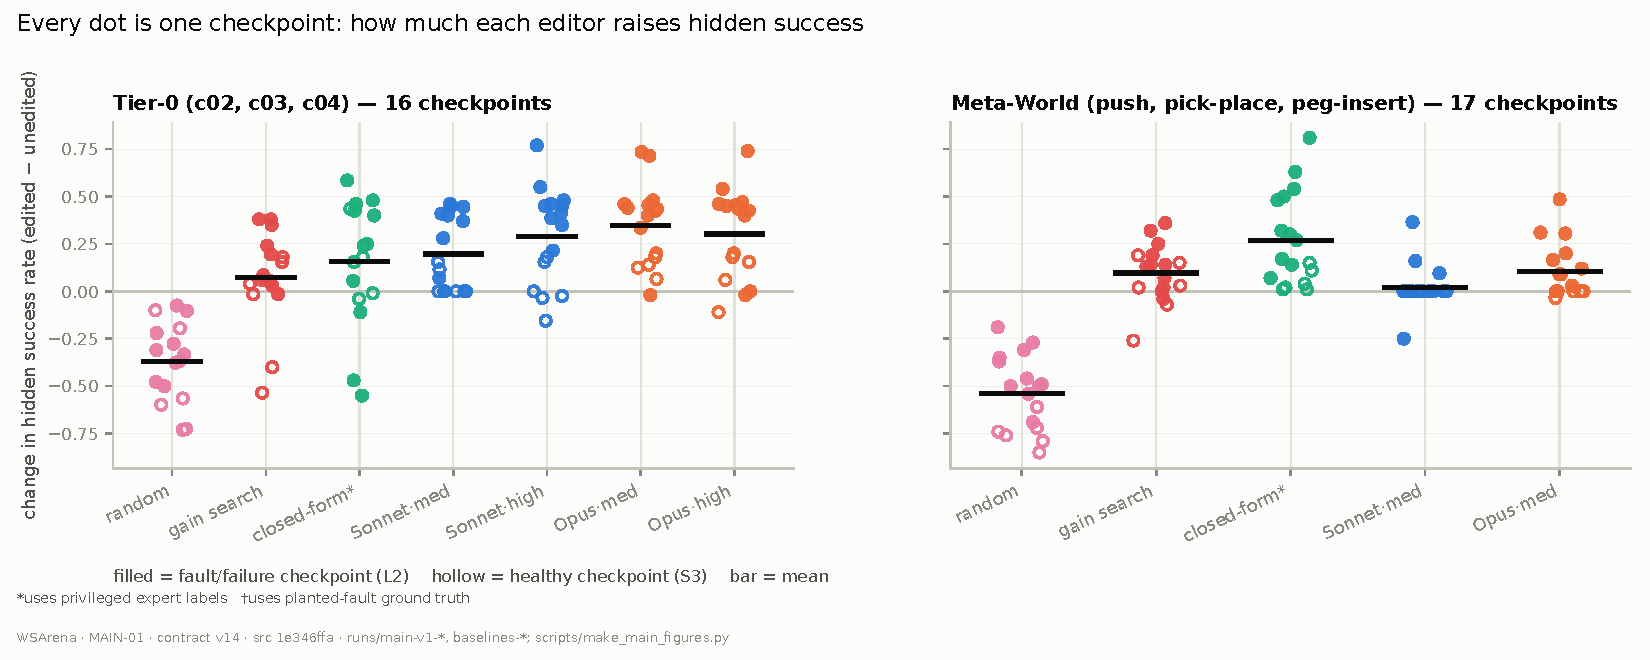
\includegraphics[width=\textwidth]{figs/MAIN-01.pdf}
\caption{Every dot is one checkpoint. Filled dots are faulty or failing checkpoints, hollow dots are healthy ones, bars are means. *The closed-form refit uses expert labels.}
\label{fig:main}
\end{figure*}

On Meta-World, abstention explains Sonnet's result but not Opus's. Sonnet submitted no valid edit in any round in 7 of 17 runs (41\%) and finished with weights identical to the start in 13 of 17 (76\%); its regression rate (successes broken by an edit) is about 0.07. Opus never abstained completely and still finished unchanged in 7 of 17 runs (41\%), yet it remains 0.22 below the closed-form refit. Reporting the attempt rate next to the gain keeps a model that does not try from looking like one that fails.

\subsection{Do the models use the weights?}
This ablation was written after the primary analysis and is exploratory. In the blind condition the weight values are removed from the prompt and everything else is unchanged. On eight control-suite checkpoints and two models (16 pairs, which are not independent) the mean difference in gain between the full and the blind prompt is $+0.006$; the checkpoint-clustered 95\% interval is $-0.115$ to $+0.115$, as wide as the 0.10 band we call indistinguishable, and no equivalence margin was set in advance. A pilot on seed-1 checkpoints gave $-0.007$. The average hides large differences of both signs (Figure~\ref{fig:wri}): 6 of 16 pairs differ by 0.05 or less, 4 differ by 0.20 or more. On the delay task the models do better with the weights; on one avoid checkpoint they do much better without them. Blind runs change more of the network (0.64 of the weights against 0.33 on the matched set), so the prompt changes the editor's behaviour as well as its information. We conclude only that we found no average benefit from seeing the values on these checkpoints. We did not ablate the feedback or the task description. An independent reproduction of the original language-model edit found a related pattern: the gain appeared only with the model's thinking mode on and came almost entirely from answers that stopped looping~\cite{playground2026robotics}.

\begin{figure}[t]
\centering
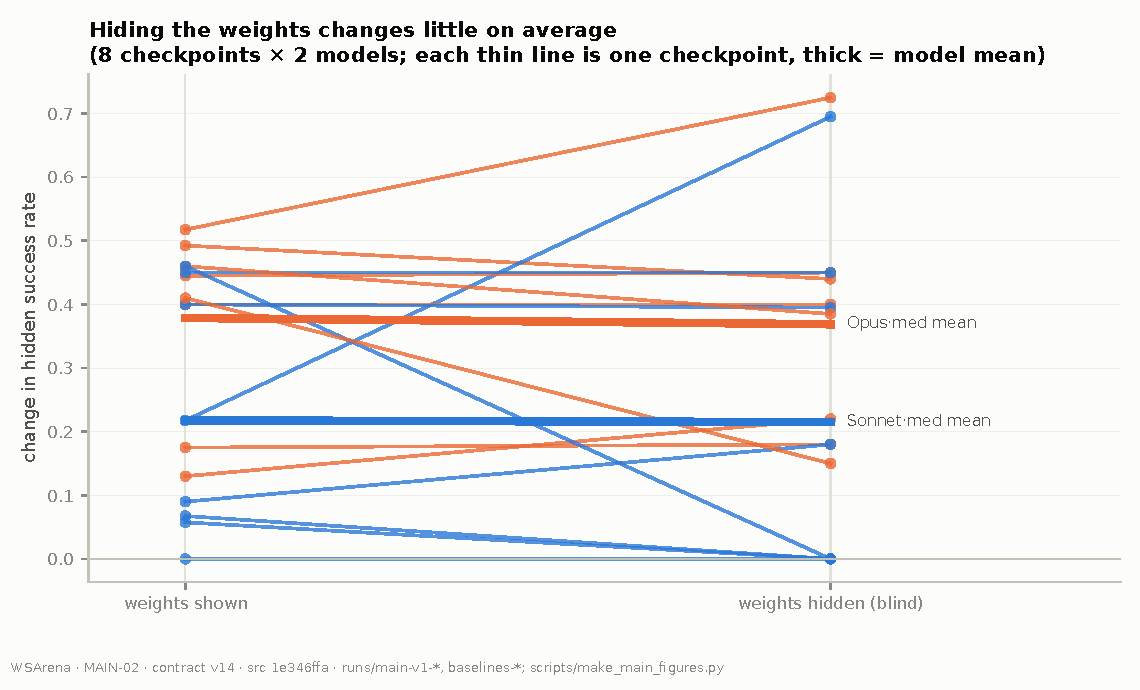
\includegraphics[width=\columnwidth]{figs/MAIN-02.pdf}
\caption{Hiding the weights changes the gain little on average (8 checkpoints, 2 models).}
\label{fig:wri}
\end{figure}

\subsection{How much do runs differ?}
These diagnostics are exploratory. For two independent runs of the same editor on the same checkpoint and prompt, the run-to-run standard deviation is 0.129 on the control suite (95\% bootstrap interval 0.05 to 0.19) and 0.078 on Meta-World (0.02 to 0.12); the two intervals overlap. The root-mean-square difference between two runs is 0.18 and 0.11, and 31\% and 19\% of pairs differ by 0.10 or more (Figure~\ref{fig:rr}). The distribution has heavy tails: without the two largest pairs the standard deviations fall to 0.07 and 0.03, and Opus on the control suite has two pairs that differ by 0.44. Test-retest correlation is 0.67 and 0.27. On Meta-World 10 of 17 checkpoints give both editors a gain below 0.10, mostly because neither edits. Rankings of the four control-suite editors agree between random halves of the checkpoints only moderately (Kendall $\tau=0.59$). The benchmark separates good editors from bad ones, but a single run should not be used to order close neighbours.

\begin{figure}[t]
\centering
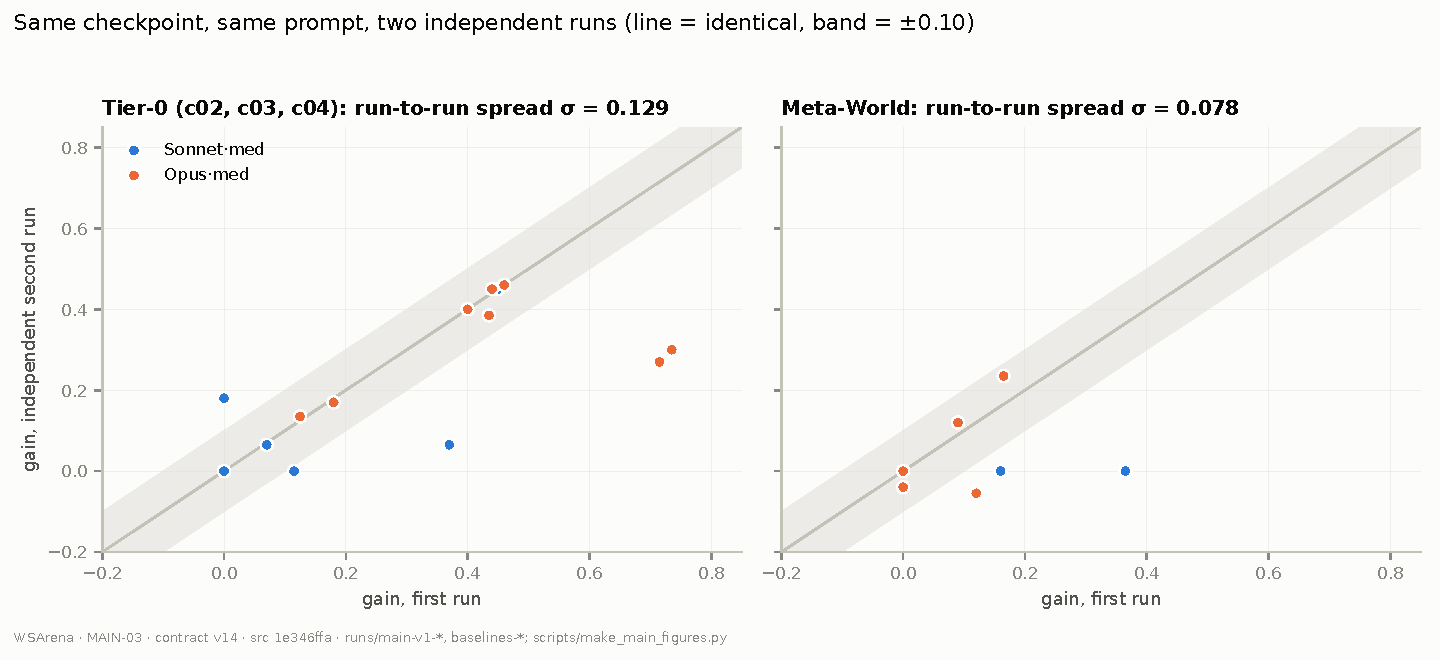
\includegraphics[width=\columnwidth]{figs/MAIN-03.pdf}
\caption{Same checkpoint, same prompt, two independent runs.}
\label{fig:rr}
\end{figure}

\subsection{Scale and probes}
\textit{TODO (runs pending): hidden width 64 and 128 with full weights, and the probe track at width 256 and 512.} Printing the weights of the width-256 policy needs about 246\,000 tokens and the width-512 policy about 982\,000, more than a typical context (Figure~\ref{fig:scale}); the probe track gives the model read-only slices, statistics and forward passes instead.

\begin{figure}[t]
\centering
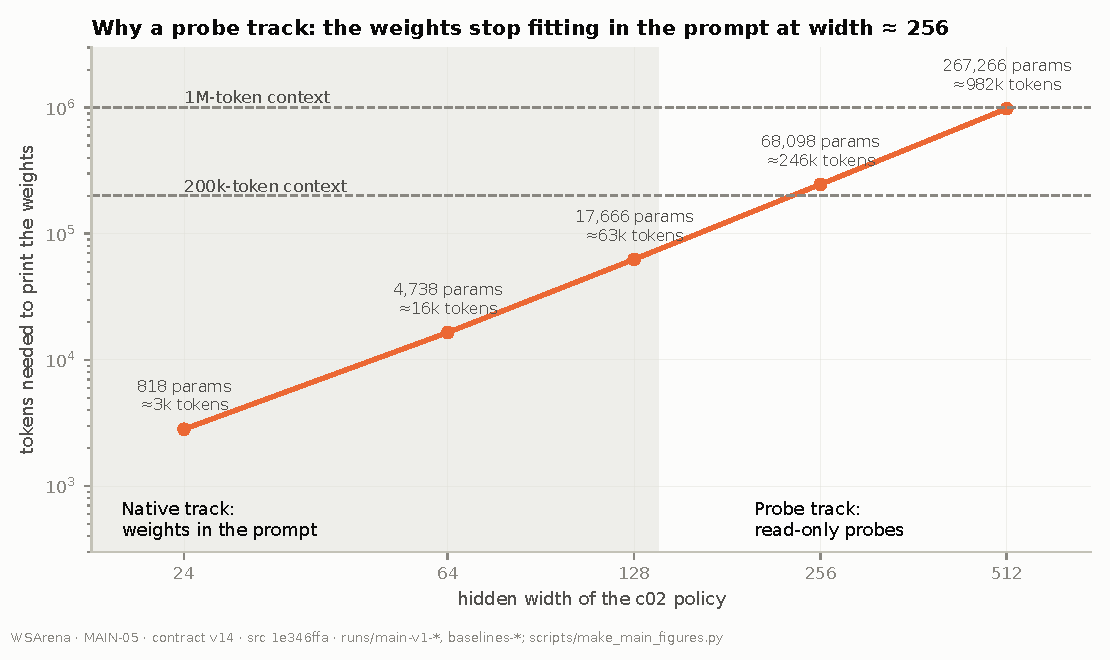
\includegraphics[width=\columnwidth]{figs/MAIN-05.pdf}
\caption{Tokens needed to print the weights of the avoid policy as a function of hidden width.}
\label{fig:scale}
\end{figure}

\section{Discussion}
\textbf{What the results say.} Editors improve faulty policies reliably, and in our exploratory ablation we found no average dependence on reading the weights. The improvement is not specific to language models: on the control suite we could not distinguish the editors from a closed-form refit, and on Meta-World the refit is clearly better. The official-benchmark tier is the more conservative of the two and should carry the headline.

\textbf{What they do not say.} The results do not show that a model understands weights, do not extend to other models, and say nothing about networks larger than a few thousand parameters until the scale and probe runs are in. They come from one task family per tier and from two models at medium effort in the second tier.

\textbf{Limitations.} Run-to-run noise limits what a single run can show; we report cluster-level estimates with intervals for that reason. Several checkpoints are at a floor, where no current editor gains anything; we keep them because they will matter for stronger models, and report them separately. The output cap we requested (64\,000 tokens) could not be verified from the client; no round was truncated.

\section{Conclusion}
WSArena measures whether a model can fix a network by writing its weights, against controls and with the noise made visible. For two current models the answer is yes, to a degree that a simple closed-form refit matches (control suite, not distinguishable) or beats (Meta-World), and we found no evidence that reading the weights is what helps. The next tests are scale and probes, which we are running.

\bibliographystyle{IEEEtran}
\bibliography{refs}
\end{document}
